\documentclass{ximera}

\title{Het SI-stelsel en prefixen}
\author{Daan Lipkens}

\begin{document}
\begin{abstract}
    De zeven basiseenheden en het werken met machten van tien.
\end{abstract}
\maketitle

\section{Het SI-stelsel}
Het SI-stelsel bestaat uit zeven basiseenheden waaruit alle andere eenheden opgebouwd kunnen worden. Deze basiseenheden worden in onderstaande tabel getoond.

\begin{center}
    \begin{tabular}{ |c|c|l| } 
    \hline
    \textbf{Symbool} & \textbf{Naam} & \textbf{Grootheid} \\
    \hline
    s & Seconde & Tijd \\
    \hline
    m & Meter & Lengte \\
    \hline
    kg & Kilogram & Massa \\
    \hline
    A & Ampère & Elektrische stroomsterkte \\
    \hline
    K & Kelvin & (Absolute) temperatuur \\
    \hline
    mol & Mol & Hoeveelheid stof \\
    \hline
    cd & Candela & Lichtsterkte \\
    \hline
    \end{tabular}
\end{center}

Al de andere eenheden die je kent zoals bijvoorbeeld snelheid, kracht,... kan je bekomen door twee of meerdere basiseenheden te combineren met mekaar.

\begin{example}[title={Gemiddelde Snelheid}]\nl
    De (gemiddelde) snelheid $v$ kan je berekenen aan de hand van de formule:
    \[ v = \frac{\Delta x}{\Delta t} \]
    Zo weet je dat $\Delta x$ een afstand is en dus uitgedrukt kan worden in meter ($\mathrm{m}$). De $\Delta t$ daarentegen is een tijd en kan dus uitgedrukt worden in seconden ($\mathrm{s}$). Om de (gemiddelde) snelheid $v$ te bekomen, deel je $\Delta x$ door $\Delta t$ waardoor je voor de eenheden van $v$ ook de eenheid van $\Delta x$ ($\mathrm{m}$) moet delen door de eenheid van $\Delta t$ ($\mathrm{s}$). Zo vind je dat $v$ uitgedrukt kan worden in $\mathrm{\frac{m}{s}}$ (of $\mathrm{m/s}$), wat je leest als meter per seconde.
\end{example}

\section{SI-prefixen}
De meter mag dan wel de basiseenheid van lengte zijn in het SI-stelsel, maar vaak is deze eenheid te groot of te klein om te gebruiken in het dagelijkse leven. Denk maar bijvoorbeeld wanneer je op reis gaat: De afstand tot je bestemming zal je nagenoeg altijd in kilometer uitdrukken, en niet in meter, omdat de meter voor deze afstanden een veel te kleine eenheid is. Daarom heeft men onderstaande prefixen ingevoerd. De kleinste en grootste prefixen (zoals giga, mega, milli en micro) gaan in stappen van $1000 \, (10^{3})$. De prefixen vlak bij de eenheid (hecto, deca, deci en centi) gaan in stappen van $10 \, (10^{1})$.

\begin{center}
    \begin{tabular}{ |c|c|c|l| } 
    \hline
    \textbf{Naam} & \textbf{Symbool} & \textbf{Macht van 10} & \textbf{Decimaal} \\
    \hline
    Giga & G & $10^{9}$ & 1 000 000 000 \\
    \hline
    Mega & M & $10^{6}$ & 1 000 000 \\
    \hline
    Kilo & k & $10^{3}$ & 1 000 \\
    \hline
    Hecto & h & $10^{2}$ & 100 \\
    \hline
    Deca & da & $10^{1}$ & 10 \\
    \hline
    / & / & $10^{0}$ & 1 \\
    \hline
    Deci & d & $10^{-1}$ & 0,1 \\
    \hline
    Centi & c & $10^{-2}$ & 0,01 \\
    \hline
    Milli & m & $10^{-3}$ & 0,001 \\
    \hline
    Micro & $\mu$ & $10^{-6}$ & 0,000 001 \\
    \hline
    Nano & n & $10^{-9}$ & 0,000 000 001 \\
    \hline
    \end{tabular}
\end{center}

\begin{example}[title={Rekenen met Prefixen}]\nl
    In de tabel kan je aflezen dat kilo (k) gelijk is aan $10^{3}$. Bijgevolg is:
    \begin{itemize}
    \item $1 \, \textcolor{red}{\mathrm{k}}\mathrm{m} = 1 \cdot \textcolor{red}{10^{3}} \, \mathrm{m} = 1000 \, \mathrm{m}$
    \item $1 \, \textcolor{red}{\mathrm{k}}\mathrm{g} = 1 \cdot \textcolor{red}{10^{3}} \, \mathrm{g} = 1000 \, \mathrm{g}$
    \end{itemize}
\end{example}

\begin{example}[title={Rekenen met Prefixen}]\nl
    In de tabel kan je aflezen dat centi (c) gelijk is aan $10^{-2}$. Bijgevolg is $1 \, \textcolor{red}{\mathrm{c}}\mathrm{m} = 1 \cdot \textcolor{red}{10^{-2}} \, \mathrm{m} = 0{,}01 \, \mathrm{m}$.
\end{example}

Het is in oefeningen ontzettend belangrijk om bovenstaande tabel met prefixen ook in de omgekeerde richting te kunnen gebruiken, wat geïllustreerd wordt met onderstaand voorbeeld.

\begin{example}[foldable=true,title={Voorbeeld: Van meter naar millimeter}]\nl
    Je meet een lengte van $5{,}0 \, \mathrm{m}$. Hoeveel millimeter is dit?

    \begin{solution}\nl
    Om deze lengte van $5{,}0 \, \mathrm{m}$ om te zetten, gaan we gelijkaardig te werk zoals we bij de vorige twee voorbeelden gedaan hebben. In de tabel kunnen we immers aflezen dat milli (m) gelijk is aan $10^{-3}$. Bijgevolg is $1 \, \textcolor{red}{\mathrm{m}}\mathrm{m} = 1 \cdot \textcolor{red}{10^{-3}} \, \mathrm{m} = 0{,}001 \, \mathrm{m}$.

    Vervolgens gaan we de vergelijking omvormen zoals je gewoon bent in wiskunde:
    \begin{align*}
    1 \, \mathrm{mm} &= 1 \cdot 10^{-3} \, \mathrm{m} & \\
    \frac{1}{10^{-3}} \, \mathrm{mm} &= 1 \, \mathrm{m} & \\
    10^{3} \, \mathrm{mm} &= 1 \, \mathrm{m} & \\
    5{,}0 \cdot 10^{3} \, \mathrm{mm} &= 5{,}0 \, \mathrm{m} & (\text{\textit{Beide leden}} \cdot 5{,}0) \\
    5000 \, \mathrm{mm} &= 5{,}0 \, \mathrm{m} &
    \end{align*}
    Dus bijgevolg vinden we dat $5{,}0 \, \mathrm{m}$ gelijk is aan $5000 \, \mathrm{mm}$.
    \end{solution}
\end{example}

\begin{remark}\nl
    Om eenheden om te zetten, kan je ook steeds gebruikmaken van een tabel zoals je in de lagere school geleerd hebt.

    Stel je hebt een afstand van $3{,}4 \, \mathrm{dm}$ gemeten. Hoeveel meter is dit? Je maakt onderstaande tabel na en noteert je gemeten waarde hierin.
    \begin{center}
        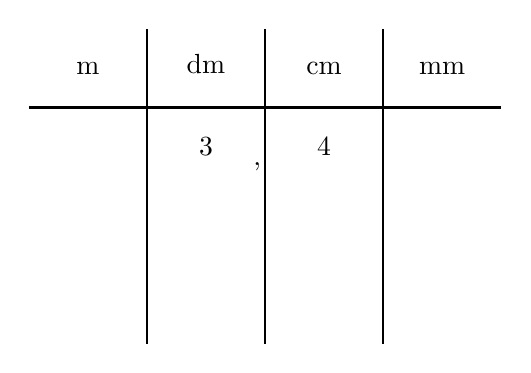
\begin{tikzpicture}[scale=1, every node/.style={scale=1}]
        \draw[color = black, smooth, thick] (0,0) -- (0,4);
        \draw[color = black, smooth, thick] (1.5,0) -- (1.5,4);
        \draw[color = black, smooth, thick] (3,0) -- (3,4);
        \draw[color = black, smooth, thick] (-1.5,3) -- (4.5,3);
        \node at (-0.75,3.5) {$\mathrm{m}$};
        \node at (0.75,3.55) {$\mathrm{dm}$};
        \node at (2.25,3.5) {$\mathrm{cm}$};
        \node at (3.75,3.5) {$\mathrm{mm}$};
        \node at (0.75,2.5) {3};
        \node at (2.25,2.5) {4};
        \node at (1.4,2.25) {,};
        \end{tikzpicture}
    \end{center}
    Je verwijdert de komma, vult aan met nullen totdat je de meter ($\mathrm{m}$) bereikt hebt en plaatst een nieuwe komma bij de rechtse verticale streep die grenst aan de kolom waarin meter genoteerd staat:
    \begin{center}
        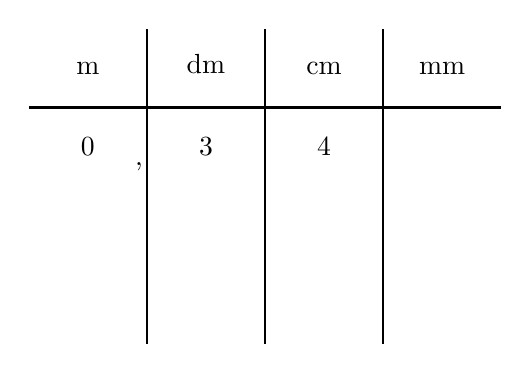
\begin{tikzpicture}[scale=1, every node/.style={scale=1}]
        \draw[color = black, smooth, thick] (0,0) -- (0,4);
        \draw[color = black, smooth, thick] (1.5,0) -- (1.5,4);
        \draw[color = black, smooth, thick] (3,0) -- (3,4);
        \draw[color = black, smooth, thick] (-1.5,3) -- (4.5,3);
        \node at (-0.75,3.5) {$\mathrm{m}$};
        \node at (0.75,3.55) {$\mathrm{dm}$};
        \node at (2.25,3.5) {$\mathrm{cm}$};
        \node at (3.75,3.5) {$\mathrm{mm}$};
        \node at (-0.75,2.5) {0};
        \node at (0.75,2.5) {3};
        \node at (2.25,2.5) {4};
        \node at (-0.1,2.25) {,};
        \end{tikzpicture}
    \end{center}
    Zo vind je dan dat $3{,}4 \, \mathrm{dm}$ gelijk is aan $0{,}34 \, \mathrm{m}$.

    \textbf{Let op!} Deze methode kan je gebruiken wanneer de sprongen in de omzettingen niet te groot zijn (bijvoorbeeld een waarde in meter, decimeter, centimeter of millimeter omzetten naar meter, decimeter, centimeter of millimeter) maar wanneer je bijvoorbeeld met micro, nano, mega of giga zit kan deze methode wel heel omslachtig zijn. Daarom is het \underline{sterk aan te raden} om eenheden met machten van 10 om te zetten zoals we gedaan hebben in de vorige voorbeelden.
\end{remark}

Tot slot, je moet niet alleen vlot eenheden naar SI-eenheden kunnen omzetten, maar je moet ook vlot kunnen wisselen tussen verschillende prefixen zoals geïllustreerd wordt in volgend voorbeeld.

\begin{example}[foldable=true,title={Voorbeeld: Kilometer naar millimeter omzetten}]\nl
    Je meet een waarde van $5{,}4 \, \mathrm{km}$. Hoeveel millimeter is dit?

    \begin{solution}\nl
    Prefix k is gelijk aan $10^{3}$ en prefix m is $10^{-3}$. Bijgevolg is:
    \begin{align*}
    1 \, \textcolor{red}{\mathrm{m}}\mathrm{m} & = 1 \cdot \textcolor{red}{10^{-3}} \, \mathrm{m} & \\
    1 \cdot 10^{6} \, \mathrm{mm} & = 1 \cdot 10^{-3} \cdot 10^{6} \, \mathrm{m} & (\text{\textit{Beide leden}} \cdot 10^{6}) \\
    1 \cdot 10^{6} \, \mathrm{mm} & = 1 \cdot \textcolor{green}{10^{3}} \, \mathrm{m} & \\
    1 \cdot 10^{6} \, \mathrm{mm} & = 1 \, \textcolor{green}{\mathrm{k}}\mathrm{m} & \\
    5{,}4 \cdot 10^{6} \, \mathrm{mm} & = 5{,}4 \, \mathrm{km} & (\text{\textit{Beide leden}} \cdot 5{,}4) \\
    \end{align*}
    \end{solution}
\end{example}

\end{document}